\chapter{Magnetic Resonance Imaging (MRI)}
\label{ch:mri}

% Chapter-opening illustrated modality infographic.
\begin{center}
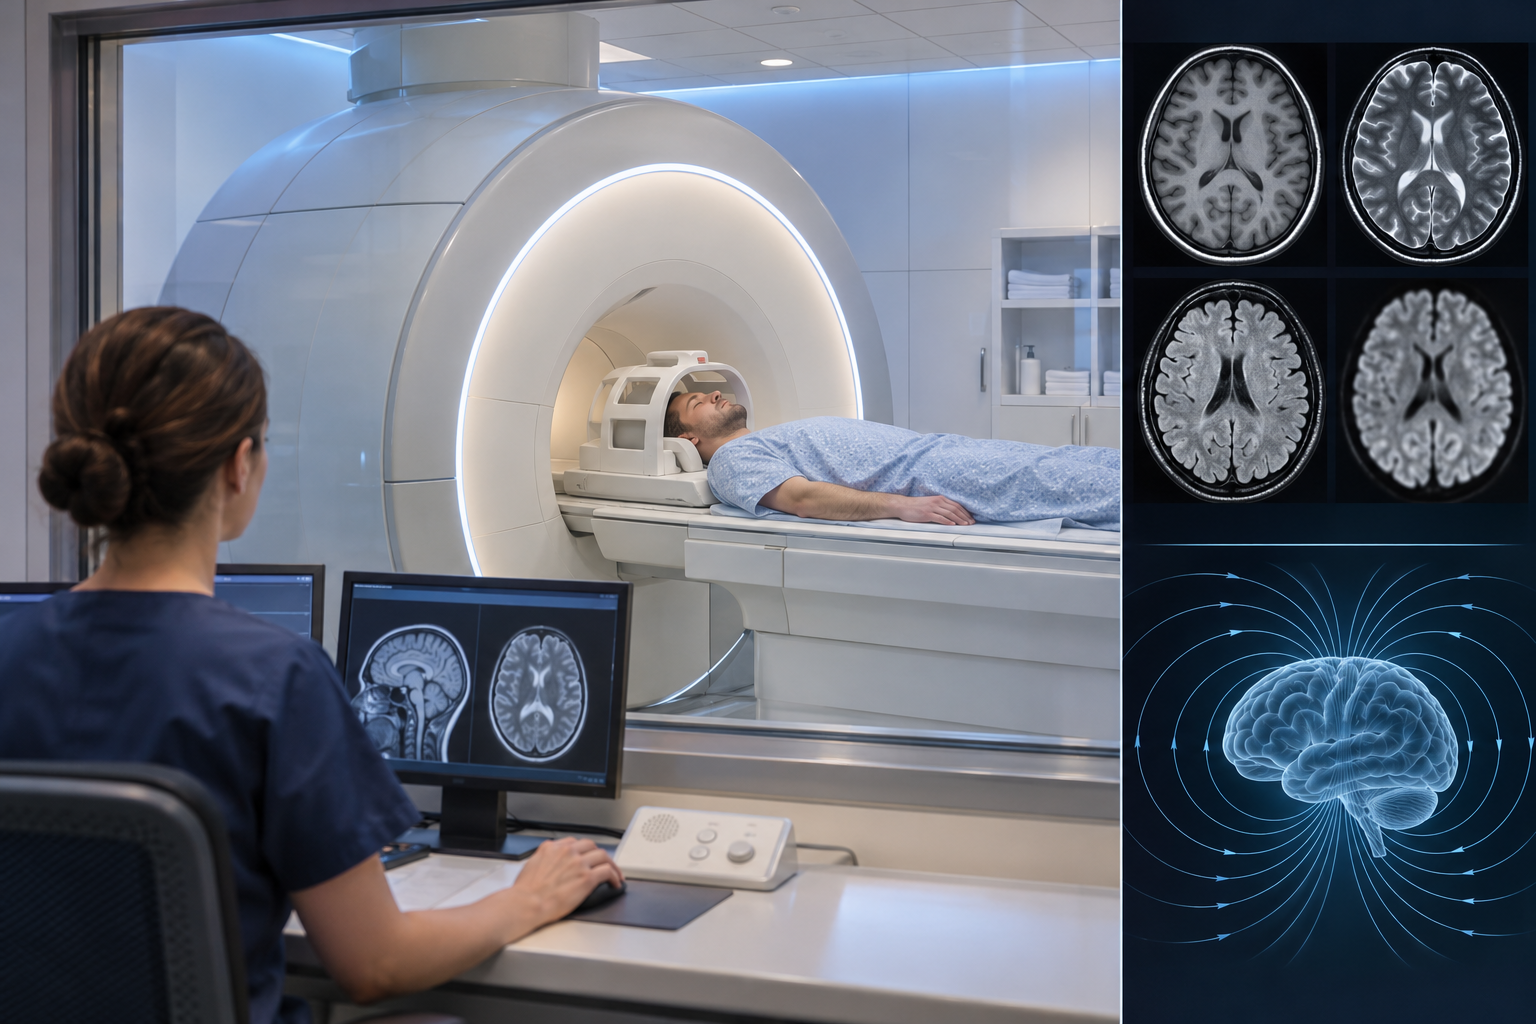
\includegraphics[width=\textwidth,keepaspectratio]{modalities/infographics/mri_realistic.png}
\end{center}
\begin{center}\footnotesize MRI uses magnetic fields and radiofrequency pulses; different sequences emphasize different tissue properties without ionizing radiation. AI-generated illustration; MRI panels are not patient studies.\end{center}

\section{Overview}
Magnetic Resonance Imaging (MRI) is a diagnostic imaging modality that uses strong magnetic fields, radiofrequency pulses, and computational reconstruction to visualize anatomical structures, tissue composition, physiological function, and blood flow.

MRI is particularly valuable for examining the brain, spinal cord, muscles, ligaments, cartilage, bone marrow, cardiovascular system, and internal organs because of its superior soft-tissue contrast.

This catalogue focuses on diseases and conditions for which MRI has established clinical diagnostic utility. It includes functional MRI (fMRI), diffusion-weighted imaging (DWI), magnetic resonance angiography (MRA), magnetic resonance venography (MRV), magnetic resonance cholangiopancreatography (MRCP), and other specialized MRI techniques.

\section{Where MRI is used}
The numbered entries below summarize characteristic MRI findings by anatomical system. Findings depend on the sequence, field strength, acquisition protocol, and clinical context; they are not, by themselves, definitive diagnoses.

\subsection{Brain and neurological disorders}
\begin{enumerate}[leftmargin=*,itemsep=0.45em,topsep=0.4em]
\item \textbf{Acute disseminated encephalomyelitis.} Useful imaging findings include: Multifocal white-matter lesions.
\item \textbf{Acute ischemic stroke.} Useful imaging findings include: Restricted diffusion on DWI.
\item \textbf{Agenesis of the corpus callosum.} Useful imaging findings include: Partial or complete absence of the corpus callosum.
\item \textbf{Alzheimer disease.} Useful imaging findings include: Medial temporal and hippocampal atrophy.
\item \textbf{Arachnoid cyst.} Useful imaging findings include: CSF-equivalent extra-axial lesion.
\item \textbf{CADASIL.} Useful imaging findings include: Anterior temporal and external capsule white-matter lesions.
\item \textbf{Central pontine myelinolysis.} Useful imaging findings include: Central pontine T2 hyperintensity.
\item \textbf{Cerebral contusion.} Useful imaging findings include: Parenchymal edema and hemorrhage.
\item \textbf{Cerebral edema.} Useful imaging findings include: Increased T2/FLAIR signal.
\item \textbf{Cerebral microbleeds.} Useful imaging findings include: Susceptibility artifacts on SWI.
\item \textbf{Cerebral small vessel disease.} Useful imaging findings include: White-matter hyperintensities, lacunes and microbleeds.
\item \textbf{Chiari malformation.} Useful imaging findings include: Cerebellar tonsillar displacement.
\item \textbf{Chronic cerebral infarction.} Useful imaging findings include: Encephalomalacia and gliosis.
\item \textbf{Creutzfeldt--Jakob disease.} Useful imaging findings include: Cortical ribboning and basal ganglia diffusion restriction.
\item \textbf{Dandy--Walker malformation.} Useful imaging findings include: Vermian abnormality and posterior fossa cystic dilatation.
\item \textbf{Diffuse axonal injury.} Useful imaging findings include: Small hemorrhagic or nonhemorrhagic white-matter lesions.
\item \textbf{Epidural hematoma.} Useful imaging findings include: Biconvex extra-axial collection.
\item \textbf{Focal cortical dysplasia.} Useful imaging findings include: Cortical thickening and blurred gray-white matter junction.
\item \textbf{Frontotemporal dementia.} Useful imaging findings include: Frontal and temporal lobe atrophy.
\item \textbf{Huntington disease.} Useful imaging findings include: Caudate nucleus atrophy.
\item \textbf{Hydrocephalus.} Useful imaging findings include: Ventricular enlargement.
\item \textbf{Hypoxic-ischemic brain injury.} Useful imaging findings include: Cortical or deep gray-matter diffusion restriction.
\item \textbf{Intracerebral hemorrhage.} Useful imaging findings include: Stage-dependent signal changes.
\item \textbf{Lissencephaly.} Useful imaging findings include: Abnormally smooth cerebral cortex.
\item \textbf{Mesial temporal sclerosis.} Useful imaging findings include: Hippocampal atrophy and increased T2 signal.
\item \textbf{MOG antibody-associated disease.} Useful imaging findings include: Inflammatory demyelinating lesions.
\item \textbf{Multiple sclerosis.} Useful imaging findings include: Periventricular, juxtacortical or infratentorial demyelinating lesions.
\item \textbf{Multiple system atrophy.} Useful imaging findings include: Pontocerebellar or putaminal abnormalities.
\item \textbf{Neuromyelitis optica spectrum disorder.} Useful imaging findings include: Characteristic optic nerve, brainstem or spinal cord lesions.
\item \textbf{Normal pressure hydrocephalus.} Useful imaging findings include: Ventriculomegaly with characteristic CSF-space distribution.
\item \textbf{Polymicrogyria.} Useful imaging findings include: Excessive small cerebral gyri.
\item \textbf{Posterior reversible encephalopathy syndrome.} Useful imaging findings include: Predominantly posterior vasogenic edema.
\item \textbf{Progressive multifocal leukoencephalopathy.} Useful imaging findings include: Asymmetric white-matter abnormalities.
\item \textbf{Progressive supranuclear palsy.} Useful imaging findings include: Midbrain atrophy, hummingbird sign.
\item \textbf{Schizencephaly.} Useful imaging findings include: Gray matter-lined cerebral cleft.
\item \textbf{Subarachnoid hemorrhage.} Useful imaging findings include: Abnormal sulcal signal on FLAIR.
\item \textbf{Subdural hematoma.} Useful imaging findings include: Crescent-shaped extra-axial collection.
\item \textbf{Vascular dementia.} Useful imaging findings include: Multiple infarcts and white-matter abnormalities.
\item \textbf{Wernicke encephalopathy.} Useful imaging findings include: Abnormal signal in medial thalami and mammillary bodies.
\item \textbf{Wilson disease.} Useful imaging findings include: Basal ganglia signal abnormalities.
\end{enumerate}

For acute intracranial hemorrhage or suspected subarachnoid hemorrhage, noncontrast CT is commonly the initial examination in emergency care. MRI can provide complementary information, and the appropriate test depends on timing and clinical circumstances.

\subsection{Brain tumors}
\begin{enumerate}[leftmargin=*,itemsep=0.45em,topsep=0.4em]
\item \textbf{Astrocytoma.} Useful imaging findings include: Infiltrative T2/FLAIR hyperintense lesion.
\item \textbf{Brain metastases.} Useful imaging findings include: Enhancing lesions with surrounding vasogenic edema.
\item \textbf{Central neurocytoma.} Useful imaging findings include: Intraventricular mass.
\item \textbf{Choroid plexus papilloma.} Useful imaging findings include: Enhancing intraventricular mass.
\item \textbf{Craniopharyngioma.} Useful imaging findings include: Solid-cystic suprasellar mass.
\item \textbf{Dermoid cyst.} Useful imaging findings include: Fat-containing intracranial lesion.
\item \textbf{Dysembryoplastic neuroepithelial tumor.} Useful imaging findings include: Multinodular cortical lesion.
\item \textbf{Ependymoma.} Useful imaging findings include: Ventricular-associated mass.
\item \textbf{Epidermoid cyst.} Useful imaging findings include: Restricted diffusion within a CSF-like lesion.
\item \textbf{Ganglioglioma.} Useful imaging findings include: Cortical solid-cystic lesion.
\item \textbf{Glioblastoma.} Useful imaging findings include: Irregular enhancement, necrosis and surrounding edema.
\item \textbf{Hemangioblastoma.} Useful imaging findings include: Hypervascular mural nodule with associated cyst.
\item \textbf{Medulloblastoma.} Useful imaging findings include: Posterior fossa mass with restricted diffusion.
\item \textbf{Meningioma.} Useful imaging findings include: Enhancing extra-axial mass, possible dural tail.
\item \textbf{Oligodendroglioma.} Useful imaging findings include: Cortical-subcortical infiltrative mass.
\item \textbf{Pilocytic astrocytoma.} Useful imaging findings include: Cystic lesion with enhancing mural nodule.
\item \textbf{Pineal region tumor.} Useful imaging findings include: Pineal region mass.
\item \textbf{Pituitary adenoma.} Useful imaging findings include: Sellar mass with variable enhancement.
\item \textbf{Primary CNS lymphoma.} Useful imaging findings include: Enhancing mass with restricted diffusion.
\item \textbf{Vestibular schwannoma.} Useful imaging findings include: Enhancing internal auditory canal or cerebellopontine angle mass.
\end{enumerate}

\subsection{Central nervous system infections}
\begin{enumerate}[leftmargin=*,itemsep=0.45em,topsep=0.4em]
\item \textbf{Bacterial meningitis.} Useful imaging findings include: Leptomeningeal enhancement.
\item \textbf{Cerebral abscess.} Useful imaging findings include: Ring enhancement with central diffusion restriction.
\item \textbf{Cerebral toxoplasmosis.} Useful imaging findings include: Multiple ring-enhancing lesions.
\item \textbf{Herpes simplex encephalitis.} Useful imaging findings include: Temporal and insular signal abnormalities.
\item \textbf{Intracranial tuberculoma.} Useful imaging findings include: Nodular or ring-enhancing lesions.
\item \textbf{Neurocysticercosis.} Useful imaging findings include: Cystic lesions, sometimes with an identifiable scolex.
\item \textbf{Subdural empyema.} Useful imaging findings include: Extra-axial collection with restricted diffusion.
\item \textbf{Tuberculous meningitis.} Useful imaging findings include: Basal meningeal enhancement.
\item \textbf{Ventriculitis.} Useful imaging findings include: Ventricular debris and ependymal enhancement.
\item \textbf{Viral encephalitis.} Useful imaging findings include: Regional or multifocal T2/FLAIR abnormalities.
\end{enumerate}

\subsection{Spine and spinal cord}
\begin{enumerate}[leftmargin=*,itemsep=0.45em,topsep=0.4em]
\item \textbf{Cauda equina syndrome.} Useful imaging findings include: Compression of cauda equina nerve roots.
\item \textbf{Cervical disc herniation.} Useful imaging findings include: Disc displacement with possible neural compression.
\item \textbf{Cervical spondylotic myelopathy.} Useful imaging findings include: Spinal cord compression and signal abnormalities.
\item \textbf{Degenerative disc disease.} Useful imaging findings include: Reduced disc hydration and height.
\item \textbf{Discitis.} Useful imaging findings include: Abnormal disc and adjacent endplate signal.
\item \textbf{Hydromyelia.} Useful imaging findings include: Dilatation of the central spinal canal.
\item \textbf{Lumbar disc herniation.} Useful imaging findings include: Displaced intervertebral disc material.
\item \textbf{Meningocele.} Useful imaging findings include: Herniation of meninges.
\item \textbf{Multiple sclerosis of the spinal cord.} Useful imaging findings include: Focal intramedullary demyelinating lesions.
\item \textbf{Myelomeningocele.} Useful imaging findings include: Herniation of meninges and neural tissue.
\item \textbf{Neural foraminal stenosis.} Useful imaging findings include: Narrowing of neural foramina.
\item \textbf{Spina bifida.} Useful imaging findings include: Posterior vertebral defect.
\item \textbf{Spinal arachnoid cyst.} Useful imaging findings include: CSF-equivalent cystic lesion.
\item \textbf{Spinal astrocytoma.} Useful imaging findings include: Infiltrative intramedullary mass.
\item \textbf{Spinal canal stenosis.} Useful imaging findings include: Narrowing of the spinal canal.
\item \textbf{Spinal cord infarction.} Useful imaging findings include: Intramedullary diffusion restriction.
\item \textbf{Spinal cord injury.} Useful imaging findings include: Cord edema, hemorrhage or disruption.
\item \textbf{Spinal ependymoma.} Useful imaging findings include: Enhancing intramedullary mass.
\item \textbf{Spinal epidural abscess.} Useful imaging findings include: Enhancing epidural collection.
\item \textbf{Spinal epidural hematoma.} Useful imaging findings include: Epidural blood collection.
\item \textbf{Spinal meningioma.} Useful imaging findings include: Enhancing intradural extramedullary mass.
\item \textbf{Spinal metastases.} Useful imaging findings include: Abnormal marrow replacement.
\item \textbf{Spinal schwannoma.} Useful imaging findings include: Nerve root-associated mass.
\item \textbf{Spinal tuberculosis.} Useful imaging findings include: Vertebral destruction and paravertebral collections.
\item \textbf{Spondylolisthesis.} Useful imaging findings include: Vertebral displacement.
\item \textbf{Syringomyelia.} Useful imaging findings include: Fluid-filled cavity within the spinal cord.
\item \textbf{Tethered cord syndrome.} Useful imaging findings include: Low-lying conus and associated tethering structures.
\item \textbf{Transverse myelitis.} Useful imaging findings include: Intramedullary T2 hyperintensity.
\item \textbf{Vertebral compression fracture.} Useful imaging findings include: Vertebral height loss and marrow edema when acute.
\item \textbf{Vertebral osteomyelitis.} Useful imaging findings include: Vertebral marrow edema and enhancement.
\end{enumerate}

\subsection{Head, neck and ophthalmology}
\begin{enumerate}[leftmargin=*,itemsep=0.45em,topsep=0.4em]
\item \textbf{Branchial cleft cyst.} Useful imaging findings include: Lateral cervical cystic lesion.
\item \textbf{Cholesteatoma.} Useful imaging findings include: Restricted diffusion on dedicated sequences.
\item \textbf{Facial nerve schwannoma.} Useful imaging findings include: Enhancing lesion along the facial nerve.
\item \textbf{Laryngeal carcinoma.} Useful imaging findings include: Abnormal laryngeal soft tissue and local invasion.
\item \textbf{Nasopharyngeal carcinoma.} Useful imaging findings include: Infiltrative nasopharyngeal mass.
\item \textbf{Optic nerve glioma.} Useful imaging findings include: Fusiform optic nerve enlargement.
\item \textbf{Optic nerve sheath meningioma.} Useful imaging findings include: Tram-track enhancement.
\item \textbf{Optic neuritis.} Useful imaging findings include: Optic nerve swelling and enhancement.
\item \textbf{Orbital abscess.} Useful imaging findings include: Rim-enhancing orbital collection.
\item \textbf{Orbital cavernous venous malformation.} Useful imaging findings include: Well-defined enhancing orbital mass.
\item \textbf{Orbital cellulitis.} Useful imaging findings include: Orbital inflammatory signal abnormalities.
\item \textbf{Paraganglioma.} Useful imaging findings include: Hypervascular mass, possible salt-and-pepper appearance.
\item \textbf{Parotid pleomorphic adenoma.} Useful imaging findings include: Typically T2 hyperintense lobulated mass.
\item \textbf{Retinoblastoma.} Useful imaging findings include: Enhancing intraocular mass.
\item \textbf{Temporomandibular joint internal derangement.} Useful imaging findings include: Abnormal articular disc position.
\item \textbf{Thyroid eye disease.} Useful imaging findings include: Extraocular muscle enlargement.
\item \textbf{Tongue carcinoma.} Useful imaging findings include: Abnormal enhancing soft-tissue mass.
\item \textbf{Trigeminal neurovascular compression.} Useful imaging findings include: Vascular contact with associated nerve deformation.
\item \textbf{Uveal melanoma.} Useful imaging findings include: Often T1 hyperintense and T2 hypointense mass.
\item \textbf{Warthin tumor.} Useful imaging findings include: Parotid mass with characteristic diffusion and enhancement features.
\end{enumerate}

\subsection{Cardiovascular system: cardiac MRI}
\begin{enumerate}[leftmargin=*,itemsep=0.45em,topsep=0.4em]
\item \textbf{Acute myocardial infarction.} Useful imaging findings include: Myocardial edema and ischemic-pattern enhancement.
\item \textbf{Arrhythmogenic cardiomyopathy.} Useful imaging findings include: Regional ventricular dysfunction and structural abnormalities.
\item \textbf{Cardiac amyloidosis.} Useful imaging findings include: Diffuse enhancement and increased extracellular volume.
\item \textbf{Cardiac angiosarcoma.} Useful imaging findings include: Heterogeneous infiltrative cardiac mass.
\item \textbf{Cardiac fibroma.} Useful imaging findings include: Intramyocardial mass with prominent delayed enhancement.
\item \textbf{Cardiac hemochromatosis.} Useful imaging findings include: Reduced myocardial T2*.
\item \textbf{Cardiac myxoma.} Useful imaging findings include: Intracavitary mass with variable tissue signal.
\item \textbf{Cardiac sarcoidosis.} Useful imaging findings include: Patchy nonischemic myocardial enhancement.
\item \textbf{Chronic myocardial infarction.} Useful imaging findings include: Subendocardial or transmural scar.
\item \textbf{Congenital heart disease.} Useful imaging findings include: Abnormal cardiac anatomy and flow.
\item \textbf{Constrictive pericarditis.} Useful imaging findings include: Pericardial abnormalities and ventricular interdependence.
\item \textbf{Dilated cardiomyopathy.} Useful imaging findings include: Ventricular dilatation and systolic dysfunction.
\item \textbf{Endomyocardial fibrosis.} Useful imaging findings include: Subendocardial fibrosis and apical obliteration.
\item \textbf{Fabry cardiomyopathy.} Useful imaging findings include: Reduced native T1 and characteristic fibrosis.
\item \textbf{Hypertrophic cardiomyopathy.} Useful imaging findings include: Myocardial hypertrophy and possible fibrosis.
\item \textbf{Intracardiac thrombus.} Useful imaging findings include: Typically nonenhancing intracardiac mass.
\item \textbf{Left ventricular aneurysm.} Useful imaging findings include: Dyskinetic ventricular outpouching.
\item \textbf{Left ventricular noncompaction phenotype.} Useful imaging findings include: Prominent myocardial trabeculation; morphology alone is insufficient to diagnose cardiomyopathy and requires clinical and functional correlation.
\item \textbf{Left ventricular pseudoaneurysm.} Useful imaging findings include: Contained ventricular rupture.
\item \textbf{Myocardial ischemia.} Useful imaging findings include: Stress-induced perfusion defect.
\item \textbf{Myocarditis.} Useful imaging findings include: Myocardial edema and nonischemic injury pattern.
\item \textbf{Pericardial effusion.} Useful imaging findings include: Fluid surrounding the heart.
\item \textbf{Pericarditis.} Useful imaging findings include: Pericardial edema and enhancement.
\item \textbf{Restrictive cardiomyopathy.} Useful imaging findings include: Abnormal ventricular filling and tissue characteristics.
\item \textbf{Takotsubo cardiomyopathy.} Useful imaging findings include: Regional ballooning and myocardial edema.
\end{enumerate}

\subsection{Vascular diseases: MRA and MRV}
\begin{enumerate}[leftmargin=*,itemsep=0.45em,topsep=0.4em]
\item \textbf{Aortic aneurysm.} Useful imaging findings include: Aortic dilatation.
\item \textbf{Aortic coarctation.} Useful imaging findings include: Focal aortic narrowing.
\item \textbf{Aortic dissection.} Useful imaging findings include: Intimal flap and separate vascular lumens.
\item \textbf{Carotid artery dissection.} Useful imaging findings include: Mural hematoma and luminal abnormality.
\item \textbf{Carotid artery stenosis.} Useful imaging findings include: Luminal narrowing.
\item \textbf{Cerebral arterial occlusion.} Useful imaging findings include: Interrupted arterial flow signal.
\item \textbf{Cerebral arterial stenosis.} Useful imaging findings include: Reduced arterial luminal diameter.
\item \textbf{Cerebral arteriovenous malformation.} Useful imaging findings include: Abnormal vascular nidus and flow.
\item \textbf{Cerebral venous sinus thrombosis.} Useful imaging findings include: Abnormal venous signal or filling defect.
\item \textbf{Deep vein thrombosis.} Useful imaging findings include: Venous filling defect on selected MRV examinations, particularly for pelvic or central veins; ultrasound is generally first-line for suspected lower-extremity DVT.
\item \textbf{Dural arteriovenous fistula.} Useful imaging findings include: Abnormal arteriovenous shunting.
\item \textbf{Fibromuscular dysplasia.} Useful imaging findings include: Irregular arterial narrowing and dilatation.
\item \textbf{Intracranial aneurysm.} Useful imaging findings include: Focal arterial outpouching.
\item \textbf{Large-vessel vasculitis.} Useful imaging findings include: Vessel wall thickening and enhancement.
\item \textbf{Moyamoya disease.} Useful imaging findings include: Intracranial arterial narrowing and collateral vessels.
\item \textbf{Peripheral arterial disease.} Useful imaging findings include: Peripheral arterial stenosis or occlusion.
\item \textbf{Popliteal artery entrapment syndrome.} Useful imaging findings include: Abnormal musculovascular anatomy or compression.
\item \textbf{Renal artery stenosis.} Useful imaging findings include: Narrowing of the renal artery.
\item \textbf{Vascular malformation.} Useful imaging findings include: Abnormal vascular channels.
\item \textbf{Vertebral artery dissection.} Useful imaging findings include: Abnormal vessel wall and lumen.
\end{enumerate}

\subsection{Liver}
\begin{enumerate}[leftmargin=*,itemsep=0.45em,topsep=0.4em]
\item \textbf{Budd--Chiari syndrome.} Useful imaging findings include: Hepatic venous obstruction.
\item \textbf{Focal nodular hyperplasia.} Useful imaging findings include: Arterial enhancement and possible hepatobiliary contrast uptake.
\item \textbf{Hepatic adenoma.} Useful imaging findings include: Variable fat, hemorrhage and enhancement.
\item \textbf{Hepatic hemangioma.} Useful imaging findings include: Marked T2 hyperintensity and characteristic enhancement.
\item \textbf{Hepatic infarction.} Useful imaging findings include: Regional perfusion and signal abnormalities.
\item \textbf{Hepatic iron overload.} Useful imaging findings include: Reduced T2/T2* signal.
\item \textbf{Hepatic metastases.} Useful imaging findings include: Focal lesions with variable enhancement and diffusion restriction.
\item \textbf{Hepatic steatosis.} Useful imaging findings include: Signal loss on opposed-phase imaging or increased MRI-PDFF.
\item \textbf{Hepatocellular carcinoma.} Useful imaging findings include: Arterial hyperenhancement and subsequent washout in appropriate cases.
\item \textbf{Hydatid cyst.} Useful imaging findings include: Daughter cysts and internal membranes.
\item \textbf{Intrahepatic cholangiocarcinoma.} Useful imaging findings include: Progressive delayed enhancement.
\item \textbf{Liver abscess.} Useful imaging findings include: Rim enhancement and possible diffusion restriction.
\item \textbf{Liver cirrhosis.} Useful imaging findings include: Nodular contour and architectural distortion.
\item \textbf{Liver fibrosis.} Useful imaging findings include: Increased stiffness on MR elastography.
\item \textbf{Polycystic liver disease.} Useful imaging findings include: Multiple hepatic cysts.
\item \textbf{Portal vein thrombosis.} Useful imaging findings include: Abnormal portal venous signal or filling defect.
\item \textbf{Simple hepatic cyst.} Useful imaging findings include: T2 hyperintense nonenhancing lesion.
\end{enumerate}

\subsection{Gallbladder and biliary system: MRCP}
\begin{enumerate}[leftmargin=*,itemsep=0.45em,topsep=0.4em]
\item \textbf{Acute cholecystitis.} Useful imaging findings include: Gallbladder wall edema and surrounding inflammation.
\item \textbf{Adenomyomatosis.} Useful imaging findings include: Intramural cystic spaces, pearl-necklace sign.
\item \textbf{Benign biliary stricture.} Useful imaging findings include: Localized ductal narrowing.
\item \textbf{Biliary atresia.} Useful imaging findings include: Abnormal or poorly visualized extrahepatic bile ducts.
\item \textbf{Biliary obstruction.} Useful imaging findings include: Proximal bile duct dilatation.
\item \textbf{Caroli disease.} Useful imaging findings include: Segmental intrahepatic ductal dilatation.
\item \textbf{Cholangiocarcinoma.} Useful imaging findings include: Biliary narrowing or enhancing mass.
\item \textbf{Choledochal cyst.} Useful imaging findings include: Cystic dilatation of the biliary tree.
\item \textbf{Choledocholithiasis.} Useful imaging findings include: Bile duct filling defects.
\item \textbf{Cholelithiasis.} Useful imaging findings include: Intraluminal gallbladder filling defects.
\item \textbf{Gallbladder carcinoma.} Useful imaging findings include: Irregular enhancing mass.
\item \textbf{Primary biliary cholangitis.} Useful imaging findings include: Possible advanced hepatic changes; often normal bile ducts.
\item \textbf{Primary sclerosing cholangitis.} Useful imaging findings include: Multifocal biliary strictures and beading.
\end{enumerate}

\subsection{Pancreas}
\begin{enumerate}[leftmargin=*,itemsep=0.45em,topsep=0.4em]
\item \textbf{Acute pancreatitis.} Useful imaging findings include: Pancreatic edema and surrounding fluid.
\item \textbf{Autoimmune pancreatitis.} Useful imaging findings include: Diffuse enlargement and characteristic enhancement.
\item \textbf{Chronic pancreatitis.} Useful imaging findings include: Ductal irregularity and parenchymal changes.
\item \textbf{Intraductal papillary mucinous neoplasm.} Useful imaging findings include: Cystic lesion communicating with pancreatic ducts.
\item \textbf{Mucinous cystic neoplasm.} Useful imaging findings include: Cystic lesion with internal septations.
\item \textbf{Necrotizing pancreatitis.} Useful imaging findings include: Nonenhancing necrotic pancreatic tissue.
\item \textbf{Pancreas divisum.} Useful imaging findings include: Abnormal pancreatic ductal configuration.
\item \textbf{Pancreatic adenocarcinoma.} Useful imaging findings include: Hypoenhancing pancreatic mass.
\item \textbf{Pancreatic neuroendocrine tumor.} Useful imaging findings include: Frequently hypervascular lesion.
\item \textbf{Pancreatic pseudocyst.} Useful imaging findings include: Encapsulated fluid collection.
\item \textbf{Serous cystadenoma.} Useful imaging findings include: Microcystic lesion.
\item \textbf{Solid pseudopapillary neoplasm.} Useful imaging findings include: Encapsulated solid-cystic mass with possible hemorrhage.
\item \textbf{Walled-off pancreatic necrosis.} Useful imaging findings include: Encapsulated collection containing necrotic material.
\end{enumerate}

\subsection{Gastrointestinal system}
\begin{enumerate}[leftmargin=*,itemsep=0.45em,topsep=0.4em]
\item \textbf{Acute appendicitis.} Useful imaging findings include: Enlarged edematous appendix.
\item \textbf{Anal carcinoma.} Useful imaging findings include: Abnormal anal canal mass.
\item \textbf{Crohn disease.} Useful imaging findings include: Bowel wall thickening, edema and hyperenhancement.
\item \textbf{Diverticulitis.} Useful imaging findings include: Inflamed diverticula and surrounding edema.
\item \textbf{Enteric fistula.} Useful imaging findings include: Abnormal communicating tract.
\item \textbf{Enterocele.} Useful imaging findings include: Small bowel descent into the pelvic floor.
\item \textbf{Gastrointestinal stromal tumor.} Useful imaging findings include: Solid or heterogeneous enhancing mass.
\item \textbf{Perianal abscess.} Useful imaging findings include: Rim-enhancing fluid collection.
\item \textbf{Perianal fistula.} Useful imaging findings include: T2 hyperintense fistulous tract.
\item \textbf{Rectal carcinoma.} Useful imaging findings include: Rectal wall mass and mesorectal involvement.
\item \textbf{Rectal prolapse.} Useful imaging findings include: Abnormal rectal descent.
\item \textbf{Rectocele.} Useful imaging findings include: Dynamic anterior rectal wall protrusion.
\item \textbf{Small bowel obstruction.} Useful imaging findings include: Dilated bowel loops and transition point.
\item \textbf{Small bowel stricture.} Useful imaging findings include: Luminal narrowing and upstream dilatation.
\item \textbf{Small bowel tumor.} Useful imaging findings include: Focal bowel mass or wall abnormality.
\item \textbf{Ulcerative colitis.} Useful imaging findings include: Continuous colonic inflammatory changes.
\end{enumerate}

\subsection{Kidneys, adrenal glands and urinary system}
\begin{enumerate}[leftmargin=*,itemsep=0.45em,topsep=0.4em]
\item \textbf{Adrenal adenoma.} Useful imaging findings include: Signal loss on opposed-phase imaging in lipid-rich lesions.
\item \textbf{Adrenal carcinoma.} Useful imaging findings include: Large heterogeneous adrenal mass.
\item \textbf{Adrenal hemorrhage.} Useful imaging findings include: Stage-dependent blood-product signal.
\item \textbf{Adrenal metastases.} Useful imaging findings include: Adrenal mass with variable signal characteristics.
\item \textbf{Adrenal myelolipoma.} Useful imaging findings include: Macroscopic fat-containing lesion.
\item \textbf{Bladder carcinoma.} Useful imaging findings include: Bladder wall mass and possible muscular invasion.
\item \textbf{Complex renal cyst.} Useful imaging findings include: Septations, mural nodules or enhancement.
\item \textbf{Hydronephrosis.} Useful imaging findings include: Dilated renal collecting system.
\item \textbf{Pheochromocytoma.} Useful imaging findings include: Variable T2 hyperintensity and enhancement.
\item \textbf{Polycystic kidney disease.} Useful imaging findings include: Multiple bilateral renal cysts.
\item \textbf{Renal abscess.} Useful imaging findings include: Rim enhancement and diffusion restriction.
\item \textbf{Renal angiomyolipoma.} Useful imaging findings include: Macroscopic or microscopic fat-related signal changes.
\item \textbf{Renal cell carcinoma.} Useful imaging findings include: Enhancing renal mass.
\item \textbf{Renal infarction.} Useful imaging findings include: Regional abnormal perfusion.
\item \textbf{Renal oncocytoma.} Useful imaging findings include: Enhancing solid renal mass.
\item \textbf{Retroperitoneal fibrosis.} Useful imaging findings include: Periaortic fibrotic soft tissue.
\item \textbf{Simple renal cyst.} Useful imaging findings include: T2 hyperintense nonenhancing lesion.
\item \textbf{Ureteropelvic junction obstruction.} Useful imaging findings include: Collecting system dilatation and junctional narrowing.
\item \textbf{Urethral diverticulum.} Useful imaging findings include: Periurethral fluid-containing structure.
\item \textbf{Urothelial carcinoma.} Useful imaging findings include: Enhancing urinary tract mass.
\end{enumerate}

\subsection{Female reproductive system}
\begin{enumerate}[leftmargin=*,itemsep=0.45em,topsep=0.4em]
\item \textbf{Adenomyosis.} Useful imaging findings include: Thickened junctional zone and myometrial cysts.
\item \textbf{Bicornuate uterus.} Useful imaging findings include: Two uterine horns and external fundal cleft.
\item \textbf{Cervical carcinoma.} Useful imaging findings include: Cervical mass and parametrial involvement.
\item \textbf{Deep infiltrating endometriosis.} Useful imaging findings include: Fibrotic infiltrative pelvic lesions.
\item \textbf{Endometrial carcinoma.} Useful imaging findings include: Endometrial mass with possible myometrial invasion.
\item \textbf{Endometriosis.} Useful imaging findings include: T1 hyperintense hemorrhagic lesions or fibrotic nodules.
\item \textbf{Hemorrhagic ovarian cyst.} Useful imaging findings include: Blood-product signal characteristics.
\item \textbf{Hydrosalpinx.} Useful imaging findings include: Dilated fluid-filled fallopian tube.
\item \textbf{Mature cystic teratoma.} Useful imaging findings include: Fat-containing adnexal lesion.
\item \textbf{Müllerian agenesis.} Useful imaging findings include: Absent or underdeveloped reproductive structures.
\item \textbf{Ovarian carcinoma.} Useful imaging findings include: Complex solid-cystic adnexal mass.
\item \textbf{Ovarian endometrioma.} Useful imaging findings include: T1 hyperintensity and T2 shading.
\item \textbf{Ovarian fibroma.} Useful imaging findings include: Typically low T2 signal.
\item \textbf{Ovarian torsion.} Useful imaging findings include: Ovarian edema and twisted vascular pedicle.
\item \textbf{Pelvic organ prolapse.} Useful imaging findings include: Dynamic descent of pelvic organs.
\item \textbf{Placenta accreta spectrum.} Useful imaging findings include: Abnormal placental morphology and uteroplacental interface.
\item \textbf{Septate uterus.} Useful imaging findings include: Internal uterine septum.
\item \textbf{Tubo-ovarian abscess.} Useful imaging findings include: Complex inflammatory adnexal mass.
\item \textbf{Unicornuate uterus.} Useful imaging findings include: Asymmetric uterine development.
\item \textbf{Uterine fibroids.} Useful imaging findings include: Typically well-defined T2 hypointense masses.
\item \textbf{Uterine leiomyosarcoma.} Useful imaging findings include: Heterogeneous mass with possible necrosis and restricted diffusion.
\item \textbf{Uterus didelphys.} Useful imaging findings include: Duplicated uterine structures.
\end{enumerate}

For acute pelvic pain, ultrasound is generally the initial examination. MRI can help when ultrasound is inconclusive, including in selected suspected torsion cases; imaging findings must not delay urgent clinical management.

\subsection{Male reproductive system}
\begin{enumerate}[leftmargin=*,itemsep=0.45em,topsep=0.4em]
\item \textbf{Benign prostatic hyperplasia.} Useful imaging findings include: Transitional-zone nodular enlargement.
\item \textbf{Penile carcinoma.} Useful imaging findings include: Infiltrative penile mass.
\item \textbf{Penile fracture.} Useful imaging findings include: Discontinuity of the tunica albuginea.
\item \textbf{Peyronie disease.} Useful imaging findings include: Fibrotic tunica albuginea plaque.
\item \textbf{Prostate carcinoma.} Useful imaging findings include: Suspicious focal signal, diffusion and enhancement abnormalities.
\item \textbf{Prostatic abscess.} Useful imaging findings include: Fluid-containing lesion with restricted diffusion.
\item \textbf{Prostatitis.} Useful imaging findings include: Variable inflammatory signal changes.
\item \textbf{Seminal vesicle cyst.} Useful imaging findings include: Cystic seminal vesicle lesion.
\item \textbf{Testicular carcinoma.} Useful imaging findings include: Solid intratesticular mass.
\item \textbf{Testicular infarction.} Useful imaging findings include: Region of reduced or absent enhancement.
\end{enumerate}

\subsection{Breast: breast MRI}
\begin{enumerate}[leftmargin=*,itemsep=0.45em,topsep=0.4em]
\item \textbf{Breast abscess.} Useful imaging findings include: Rim-enhancing fluid collection.
\item \textbf{Breast cyst.} Useful imaging findings include: T2 hyperintense nonenhancing lesion.
\item \textbf{Breast implant rupture.} Useful imaging findings include: Linguine, keyhole or other implant rupture signs.
\item \textbf{Ductal carcinoma in situ.} Useful imaging findings include: Suspicious segmental or ductal nonmass enhancement.
\item \textbf{Fat necrosis.} Useful imaging findings include: Fat-containing lesion with variable enhancement.
\item \textbf{Fibroadenoma.} Useful imaging findings include: Circumscribed enhancing mass.
\item \textbf{Inflammatory breast cancer.} Useful imaging findings include: Diffuse enhancement, skin thickening and edema.
\item \textbf{Intraductal papilloma.} Useful imaging findings include: Enhancing intraductal lesion.
\item \textbf{Invasive ductal carcinoma.} Useful imaging findings include: Irregular enhancing mass.
\item \textbf{Invasive lobular carcinoma.} Useful imaging findings include: Nonmass enhancement or infiltrative mass.
\item \textbf{Phyllodes tumor.} Useful imaging findings include: Large heterogeneous enhancing mass.
\item \textbf{Residual or recurrent breast cancer.} Useful imaging findings include: Suspicious enhancement near the treatment site.
\end{enumerate}

Breast MRI is used for selected indications, such as high-risk screening and specific diagnostic, staging, or treatment-planning questions. It does not replace mammography or targeted ultrasound for routine population screening or every breast complaint.

\subsection{Bones and bone marrow}
\begin{enumerate}[leftmargin=*,itemsep=0.45em,topsep=0.4em]
\item \textbf{Aneurysmal bone cyst.} Useful imaging findings include: Multiple fluid-fluid levels.
\item \textbf{Bone infarction.} Useful imaging findings include: Serpiginous medullary signal abnormalities.
\item \textbf{Bone lymphoma.} Useful imaging findings include: Infiltrative marrow lesion.
\item \textbf{Bone metastases.} Useful imaging findings include: Marrow-replacing lesions.
\item \textbf{Brodie abscess.} Useful imaging findings include: Intraosseous abscess, possible penumbra sign.
\item \textbf{Chondroblastoma.} Useful imaging findings include: Epiphyseal lesion with surrounding edema.
\item \textbf{Chondrosarcoma.} Useful imaging findings include: Lobulated T2 hyperintense lesion.
\item \textbf{Ewing sarcoma.} Useful imaging findings include: Infiltrative marrow lesion and soft-tissue mass.
\item \textbf{Fibrous dysplasia.} Useful imaging findings include: Variable marrow signal corresponding to fibrous tissue.
\item \textbf{Giant cell tumor.} Useful imaging findings include: Expansile marrow lesion.
\item \textbf{Multiple myeloma.} Useful imaging findings include: Focal or diffuse marrow infiltration.
\item \textbf{Occult fracture.} Useful imaging findings include: Fracture line and marrow edema.
\item \textbf{Osteochondroma.} Useful imaging findings include: Bony lesion with identifiable cartilage cap.
\item \textbf{Osteomyelitis.} Useful imaging findings include: Marrow edema and enhancement.
\item \textbf{Osteonecrosis.} Useful imaging findings include: Serpiginous marrow abnormality.
\item \textbf{Osteosarcoma.} Useful imaging findings include: Marrow-replacing mass and soft-tissue extension.
\item \textbf{Paget disease.} Useful imaging findings include: Altered bone architecture and marrow characteristics.
\item \textbf{Stress fracture.} Useful imaging findings include: Marrow edema and possible fracture line.
\item \textbf{Transient osteoporosis.} Useful imaging findings include: Diffuse bone marrow edema.
\item \textbf{Unicameral bone cyst.} Useful imaging findings include: Fluid-containing intraosseous lesion.
\end{enumerate}

\subsection{Joints and cartilage}
\begin{enumerate}[leftmargin=*,itemsep=0.45em,topsep=0.4em]
\item \textbf{Acetabular labral tear.} Useful imaging findings include: Abnormal labral signal or morphology.
\item \textbf{Adhesive capsulitis.} Useful imaging findings include: Capsular thickening and inflammatory changes.
\item \textbf{Ankylosing spondylitis.} Useful imaging findings include: Sacroiliac inflammation and structural changes.
\item \textbf{Articular cartilage defect.} Useful imaging findings include: Focal cartilage loss.
\item \textbf{Charcot arthropathy.} Useful imaging findings include: Joint destruction, fragmentation and marrow abnormalities.
\item \textbf{Femoroacetabular impingement.} Useful imaging findings include: Abnormal hip morphology and associated tissue injury.
\item \textbf{Glenoid labral tear.} Useful imaging findings include: Labral disruption.
\item \textbf{Gout.} Useful imaging findings include: Tophi and erosions.
\item \textbf{Legg--Calvé--Perthes disease.} Useful imaging findings include: Femoral head ischemia and structural abnormalities.
\item \textbf{Meniscal tear.} Useful imaging findings include: Abnormal meniscal signal reaching an articular surface.
\item \textbf{Osteoarthritis.} Useful imaging findings include: Cartilage loss and subchondral abnormalities.
\item \textbf{Osteochondral fracture.} Useful imaging findings include: Disrupted cartilage and underlying bone.
\item \textbf{Osteochondritis dissecans.} Useful imaging findings include: Subchondral osteochondral lesion.
\item \textbf{Patellar instability.} Useful imaging findings include: Patellofemoral abnormalities and associated injuries.
\item \textbf{Psoriatic arthritis.} Useful imaging findings include: Synovitis, enthesitis and marrow edema.
\item \textbf{Rheumatoid arthritis.} Useful imaging findings include: Synovitis, erosions and marrow edema.
\item \textbf{Sacroiliitis.} Useful imaging findings include: Subchondral marrow edema and erosions.
\item \textbf{Septic arthritis.} Useful imaging findings include: Joint effusion and inflammatory enhancement.
\item \textbf{Synovial chondromatosis.} Useful imaging findings include: Multiple intra-articular nodules.
\item \textbf{Tenosynovial giant cell tumor.} Useful imaging findings include: Synovial proliferation with hemosiderin-related susceptibility.
\end{enumerate}

\subsection{Ligaments, tendons and muscles}
\begin{enumerate}[leftmargin=*,itemsep=0.45em,topsep=0.4em]
\item \textbf{Achilles tendon rupture.} Useful imaging findings include: Tendon disruption and retraction.
\item \textbf{Anterior cruciate ligament tear.} Useful imaging findings include: ACL fiber disruption.
\item \textbf{Athletic pubalgia.} Useful imaging findings include: Injury of the pubic aponeurotic structures.
\item \textbf{Biceps tendon rupture.} Useful imaging findings include: Tendon discontinuity or displacement.
\item \textbf{Bursitis.} Useful imaging findings include: Fluid-filled distended bursa.
\item \textbf{De Quervain tenosynovitis.} Useful imaging findings include: First extensor compartment inflammation.
\item \textbf{Dermatomyositis.} Useful imaging findings include: Muscle and fascial edema.
\item \textbf{Inclusion body myositis.} Useful imaging findings include: Selective muscle atrophy and fatty replacement.
\item \textbf{Lateral collateral ligament tear.} Useful imaging findings include: Ligament fiber abnormality.
\item \textbf{Medial collateral ligament tear.} Useful imaging findings include: Ligament disruption and surrounding edema.
\item \textbf{Muscle hematoma.} Useful imaging findings include: Stage-dependent blood-product signal.
\item \textbf{Muscle strain.} Useful imaging findings include: Feathery intramuscular edema.
\item \textbf{Muscle tear.} Useful imaging findings include: Fiber disruption and hemorrhage.
\item \textbf{Muscular dystrophy.} Useful imaging findings include: Characteristic patterns of fatty muscle replacement.
\item \textbf{Myositis.} Useful imaging findings include: Muscle edema and enhancement.
\item \textbf{Patellar tendon rupture.} Useful imaging findings include: Patellar tendon discontinuity.
\item \textbf{Plantar fasciitis.} Useful imaging findings include: Plantar fascial thickening and edema.
\item \textbf{Posterior cruciate ligament tear.} Useful imaging findings include: PCL fiber disruption.
\item \textbf{Quadriceps tendon rupture.} Useful imaging findings include: Tendon fiber disruption.
\item \textbf{Rotator cuff tear.} Useful imaging findings include: Tendon discontinuity.
\item \textbf{Tendinopathy.} Useful imaging findings include: Tendon thickening and increased signal.
\item \textbf{Tenosynovitis.} Useful imaging findings include: Tendon sheath fluid and enhancement.
\end{enumerate}

\subsection{Peripheral nerves: MR neurography}
\begin{enumerate}[leftmargin=*,itemsep=0.45em,topsep=0.4em]
\item \textbf{Brachial plexopathy.} Useful imaging findings include: Plexus enlargement or abnormal signal.
\item \textbf{Carpal tunnel syndrome.} Useful imaging findings include: Median nerve enlargement and abnormal signal.
\item \textbf{Lumbosacral plexopathy.} Useful imaging findings include: Abnormal plexus signal.
\item \textbf{Malignant peripheral nerve sheath tumor.} Useful imaging findings include: Heterogeneous infiltrative nerve-associated mass.
\item \textbf{Morton neuroma.} Useful imaging findings include: Intermetatarsal soft-tissue mass.
\item \textbf{Neurofibroma.} Useful imaging findings include: Nerve-associated mass, possible target sign.
\item \textbf{Parsonage--Turner syndrome.} Useful imaging findings include: Nerve abnormalities and muscle denervation.
\item \textbf{Peripheral nerve injury.} Useful imaging findings include: Nerve discontinuity or edema.
\item \textbf{Peripheral nerve schwannoma.} Useful imaging findings include: Nerve-associated enhancing mass.
\item \textbf{Piriformis-related sciatic nerve entrapment.} Useful imaging findings include: Sciatic nerve signal changes or anatomical compression.
\item \textbf{Tarsal tunnel syndrome.} Useful imaging findings include: Tibial nerve abnormalities or compressing lesion.
\item \textbf{Ulnar nerve entrapment.} Useful imaging findings include: Ulnar nerve swelling and signal abnormality.
\end{enumerate}

\subsection{Soft tissues and tumors}
\begin{enumerate}[leftmargin=*,itemsep=0.45em,topsep=0.4em]
\item \textbf{Cellulitis.} Useful imaging findings include: Subcutaneous edema and enhancement.
\item \textbf{Desmoid-type fibromatosis.} Useful imaging findings include: Infiltrative fibrous soft-tissue lesion.
\item \textbf{Ganglion cyst.} Useful imaging findings include: Well-defined fluid-signal lesion.
\item \textbf{Leiomyosarcoma.} Useful imaging findings include: Heterogeneous enhancing mass.
\item \textbf{Lipoma.} Useful imaging findings include: Homogeneous fat-equivalent signal.
\item \textbf{Liposarcoma.} Useful imaging findings include: Fat-containing or heterogeneous soft-tissue mass.
\item \textbf{Lymphatic malformation.} Useful imaging findings include: Multicystic fluid-containing lesion.
\item \textbf{Necrotizing fasciitis.} Useful imaging findings include: Deep fascial edema and abnormal enhancement.
\item \textbf{Rhabdomyosarcoma.} Useful imaging findings include: Infiltrative soft-tissue mass.
\item \textbf{Soft-tissue abscess.} Useful imaging findings include: Rim enhancement and possible diffusion restriction.
\item \textbf{Soft-tissue hematoma.} Useful imaging findings include: Blood-product signal characteristics.
\item \textbf{Synovial sarcoma.} Useful imaging findings include: Heterogeneous enhancing soft-tissue mass.
\item \textbf{Venous malformation.} Useful imaging findings include: Lobulated T2 hyperintense vascular channels.
\end{enumerate}

\subsection{Fetal MRI}
\begin{enumerate}[leftmargin=*,itemsep=0.45em,topsep=0.4em]
\item \textbf{Agenesis of the corpus callosum.} Useful imaging findings include: Absent or incomplete corpus callosum.
\item \textbf{Congenital diaphragmatic hernia.} Useful imaging findings include: Abdominal organs within the fetal thorax.
\item \textbf{Congenital pulmonary airway malformation.} Useful imaging findings include: Abnormal cystic or solid lung lesion.
\item \textbf{Dandy--Walker malformation.} Useful imaging findings include: Abnormal vermis and posterior fossa structures.
\item \textbf{Fetal bowel obstruction.} Useful imaging findings include: Dilated bowel loops.
\item \textbf{Fetal cortical malformation.} Useful imaging findings include: Abnormal cortical development.
\item \textbf{Fetal intracranial hemorrhage.} Useful imaging findings include: Blood-product signal abnormalities.
\item \textbf{Fetal renal agenesis.} Useful imaging findings include: Absence of renal structures.
\item \textbf{Fetal spina bifida.} Useful imaging findings include: Spinal defect and associated abnormalities.
\item \textbf{Fetal urinary tract obstruction.} Useful imaging findings include: Urinary tract dilatation.
\item \textbf{Fetal ventriculomegaly.} Useful imaging findings include: Dilated cerebral ventricles.
\item \textbf{Holoprosencephaly.} Useful imaging findings include: Incomplete separation of cerebral hemispheres.
\item \textbf{Pulmonary sequestration.} Useful imaging findings include: Abnormal fetal lung tissue.
\item \textbf{Sacrococcygeal teratoma.} Useful imaging findings include: Solid-cystic sacrococcygeal mass.
\end{enumerate}

Fetal MRI is a supplementary examination, generally performed after ultrasound identifies or raises concern about a fetal abnormality. It is not a routine screening test.

\subsection{Summary of catalogue}
\begin{center}
\begin{tabular}{@{}p{0.70\textwidth}r@{}}
\toprule
\textbf{Disease category} & \textbf{Entries} \\
\midrule
Bones and bone marrow & 20 \\
Brain and neurological disorders & 40 \\
Brain tumors & 20 \\
Breast & 12 \\
Cardiovascular system & 25 \\
Central nervous system infections & 10 \\
Female reproductive system & 22 \\
Fetal MRI & 14 \\
Gallbladder and biliary system & 13 \\
Gastrointestinal system & 16 \\
Head, neck and ophthalmology & 20 \\
Joints and cartilage & 20 \\
Kidneys, adrenal glands and urinary system & 20 \\
Ligaments, tendons and muscles & 22 \\
Liver & 17 \\
Male reproductive system & 10 \\
Pancreas & 13 \\
Peripheral nerves & 12 \\
Soft tissues and tumors & 13 \\
Spine and spinal cord & 30 \\
Vascular diseases & 20 \\
\midrule
\textbf{Total} & \textbf{389} \\
\bottomrule
\end{tabular}
\end{center}

\subsection{MRI acquisition sequences}
MRI does not have a single standardized tissue intensity scale; an abnormality's appearance depends heavily on the acquisition sequence.
\begin{longtable}{@{}p{0.36\textwidth}p{0.58\textwidth}@{}}
\toprule
\textbf{MRI sequence} & \textbf{Primary diagnostic utility} \\
\midrule
\endfirsthead
\toprule
\textbf{MRI sequence} & \textbf{Primary diagnostic utility} \\
\midrule
\endhead
ADC mapping & Quantitative diffusion assessment \\
Arterial spin labeling (ASL) & Noncontrast tissue perfusion \\
Chemical shift imaging & Microscopic fat characterization \\
Cine MRI & Dynamic cardiac and anatomical motion \\
Diffusion tensor imaging (DTI) & White-matter fiber organization \\
DWI & Restricted diffusion, stroke and tumor assessment \\
Dynamic contrast-enhanced MRI & Tissue enhancement kinetics \\
FLAIR & Brain lesions with CSF signal suppression \\
Functional MRI (fMRI) & Brain functional mapping \\
GRE & Blood products and susceptibility abnormalities \\
MR angiography (MRA) & Arterial anatomy \\
MR elastography & Tissue stiffness and fibrosis \\
MR enterography & Small bowel abnormalities \\
MR neurography & Peripheral nerve abnormalities \\
MR spectroscopy (MRS) & Tissue metabolite characterization \\
MR venography (MRV) & Venous anatomy \\
MRCP & Pancreatic and biliary ducts \\
MRI-PDFF & Quantitative tissue fat fraction \\
Perfusion MRI & Tissue perfusion \\
Postcontrast T1 & Enhancement of tumors and inflammatory lesions \\
STIR & Fat suppression and musculoskeletal edema \\
SWI & Microhemorrhages and venous structures \\
T1 mapping & Quantitative tissue characterization \\
T1-weighted imaging & Anatomy, fat and marrow characterization \\
T2 mapping & Tissue water content and edema \\
T2* mapping & Iron deposition and susceptibility \\
T2-weighted imaging & Fluid, inflammation and edema \\
\bottomrule
\end{longtable}

\subsection{Standardized MRI reporting systems}
\begin{longtable}{@{}p{0.36\textwidth}p{0.58\textwidth}@{}}
\toprule
\textbf{Reporting system} & \textbf{Clinical application} \\
\midrule
\endfirsthead
\toprule
\textbf{Reporting system} & \textbf{Clinical application} \\
\midrule
\endhead
BI-RADS & Breast abnormalities \\
Bosniak classification & Cystic renal masses \\
LI-RADS & Liver lesions in at-risk populations \\
MET-RADS-P & Metastatic prostate cancer assessment \\
MY-RADS & Multiple myeloma assessment \\
NI-RADS & Post-treatment head and neck cancer surveillance \\
O-RADS MRI & Ovarian and adnexal lesions \\
PI-RADS & Prostate cancer \\
RANO & Brain tumor treatment response \\
VI-RADS & Bladder cancer muscle invasion \\
\bottomrule
\end{longtable}

\subsection{Published MRI images and datasets}
\begin{longtable}{@{}p{0.36\textwidth}p{0.58\textwidth}@{}}
\toprule
\textbf{Source} & \textbf{Primary utility} \\
\midrule
\endfirsthead
\toprule
\textbf{Source} & \textbf{Primary utility} \\
\midrule
\endhead
ACR Appropriateness Criteria & Clinical indications for ordering MRI \\
ADNI & Alzheimer disease and neurodegeneration \\
BraTS & Brain tumor MRI segmentation \\
fastMRI & Raw MRI acquisition and reconstruction datasets \\
Human Connectome Project & Brain anatomy and connectivity \\
Medical Segmentation Decathlon & Medical image segmentation \\
OpenNeuro & Structural and functional neuroimaging \\
Osteoarthritis Initiative & Musculoskeletal MRI \\
PubMed Central & Published clinical MRI images \\
Radiopaedia & Annotated clinical MRI cases \\
The Cancer Imaging Archive (TCIA) & Oncological MRI datasets \\
\bottomrule
\end{longtable}

\subsection{Recommended MRI dataset metadata}
\begin{longtable}{@{}p{0.45\textwidth}p{0.49\textwidth}@{}}
\toprule
\textbf{Attribute} & \textbf{Example} \\
\midrule
Acquisition sequence & T2-FLAIR \\
Anatomical region & Brain \\
Annotation & Segmentation mask \\
Contrast agent & Gadolinium-based agent, if administered \\
Diagnostic reference standard & Validated clinical diagnostic criteria \\
Disease & Multiple sclerosis \\
Echo time (TE) & 120 ms \\
Image format & DICOM or NIfTI \\
Image license & CC BY or other specified license \\
Image orientation & Axial \\
Imaging modality & MRI \\
Inversion time (TI) & 2,500 ms \\
Magnetic field strength & 3 Tesla \\
Publication reference & DOI or PMID \\
Radiological finding & Periventricular hyperintense lesions \\
Repetition time (TR) & 9,000 ms \\
Slice thickness & 1 mm \\
\bottomrule
\end{longtable}

\subsection{Selected clinical guidance}
The following resources support the modality-selection and interpretation notes in this chapter:
\begin{itemize}
\item \href{https://acsearch.acr.org/docs/69416/Narrative}{ACR Appropriateness Criteria: Suspected Lower Extremity Deep Vein Thrombosis} (ultrasound is the recommended initial examination; MRV has selected uses).
\item \href{https://acsearch.acr.org/docs/69503/narrative/}{ACR Appropriateness Criteria: Acute Pelvic Pain in the Reproductive Age Group} (ultrasound is generally initial; MRI can help in equivocal cases).
\item \href{https://acsearch.acr.org/docs/3102400/Narrative/}{ACR Appropriateness Criteria: Second and Third Trimester Screening for Fetal Anomaly} (fetal MRI is supplementary and appropriate after selected major findings on ultrasound).
\item \href{https://acsearch.acr.org/docs/3155692/Narrative}{ACR Appropriateness Criteria: Breast Cancer Screening} (MRI is used for selected risk groups, alongside mammography).
\item \href{https://www.acc.org/latest-in-cardiology/ten-points-to-remember/2023/08/30/02/53/2023-esc-guidelines-for-cardiomyopathies-esc-2023}{2023 ESC Guidelines for the Management of Cardiomyopathies} (imaging phenotype should be interpreted with clinical, family-history, and other diagnostic information).
\item \href{https://acsearch.acr.org/docs/69482/Narrative}{ACR Appropriateness Criteria: Headache} (MRI FLAIR and susceptibility sequences can show subarachnoid blood, but sulcal FLAIR signal is not specific and MRI has selected roles).
\end{itemize}

\subsection{Important considerations for medical imaging research}
MRI should be treated as a multisequence, multidimensional imaging modality rather than a collection of independent grayscale images. A comprehensive brain MRI may include T1, T2, FLAIR, DWI, ADC, SWI, and postcontrast sequences; each supplies distinct information about the same anatomy. An AI diagnostic system trained exclusively on isolated MRI images may overlook this complementary information.

